% Chapter Template

\chapter{Introduction} % Main chapter title

\label{Chapter 1} % Change X to a consecutive number; for referencing this chapter elsewhere, use \ref{ChapterX}

\lhead{Chapter 1. \emph{Introduction}} % Change X to a consecutive number; this is for the header on each page - perhaps a shortened title

%----------------------------------------------------------------------------------------
%	SECTION 1
%---------------------------------------------------------------------------------------
\section{Introduction}
      In modern automotives, use of images and videos captured by the cameras installed on the vehicle bodies is no longer limited to assisting drivers in getting a more comprehensive understanding of their surroundings as was seen previously in the case of backup cameras. Instead, multiple single shot detection (SSD) pipelines processing sensory camera inputs are executed periodically leveraging state-of-the-art convolutional neural networks (CNNs) for tasks such as object detection and course correction in autopilot mode. For sustaining simultaneous execution of such pipelines, the underlying compute hardware is being constantly redesigned for enabling support for concurrency in terms of executing multiple kernels together.

        Over the years, parallelism in GPU devices at a hardware level has seen an exponential growth. With each new micro-architecture, Nvidia has allowed greater scope for developing and deploying highly-parallel and efficient applications.
        
        However while there exists support from the hardware, software-level optimizations must also be considered in order to exploit the potential the GPU architecture efficiently.
    
    	\begin{figure}[ht] 
		\centering
		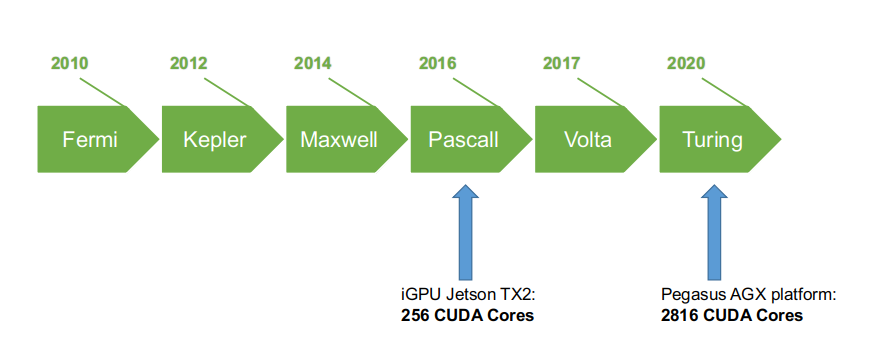
\includegraphics[scale=0.5]{Pictures/ch1/microarchitecture.png}
		\caption{CUDA micro-architectures over the years \label{fig:dagmapping}}
    \end{figure}  
    
	For example co-scheduling multiple pipelines together on the same GPU hardware would first require ascertaining the feasibility of scheduling independent kernels together since they share common memory. Thus, it becomes increasingly crucial to consider locality aware optimizations at the time of dispatching individual kernels to the GPU. 
	
	However, in order to understand the nuances of scheduling these optimized kernels, we must first understand the GPU architecture on which these kernels will be executed and the underlying programming model. Chapter 2 provides the necessary background context on CUDA, while Chapter 3 covers thread coarsening as an optimization along with discussion on the observations made over the course of the project.

   
